\documentclass[10pt]{article}

\usepackage{amsmath,amssymb,amsthm}
\usepackage{fancyhdr,url,hyperref}
\usepackage{graphicx,xspace}
\usepackage{tikz}
\usetikzlibrary{shapes,arrows,decorations.pathmorphing,backgrounds,positioning,fit,through}

\oddsidemargin 0in  %0.5in
\topmargin     0in
\leftmargin    0in
\rightmargin   0in
\textheight    9in
\textwidth     6in %6in
%\headheight    0in
%\headsep       0in
%\footskip      0.5in

\newtheorem{thm}{Theorem}
\newtheorem{cor}[thm]{Corollary}
\newtheorem{obs}{Observation}
\newtheorem{lemma}{Lemma}
\newtheorem{claim}{Claim}
\newtheorem{definition}{Definition}
\newtheorem{question}{Question}
\newtheorem{answer}{Answer}
\newtheorem{problem}{Problem}
\newtheorem{solution}{Solution}
\newtheorem{conjecture}{Conjecture}

\pagestyle{fancy}

\lhead{\textsc{Prof. McNamara}}
\chead{\textsc{SDS/MTH 291: Lecture notes}}
\lfoot{}
\cfoot{}
%\cfoot{\thepage}
\rfoot{}
\renewcommand{\headrulewidth}{0.2pt}
\renewcommand{\footrulewidth}{0.0pt}

\newcommand{\ans}{\vspace{0.25in}}
\newcommand{\R}{{\sf R}\xspace}
\newcommand{\cmd}[1]{\texttt{#1}}
\DeclareMathOperator{\Ex}{\mathbb{E}}
\DeclareMathOperator{\Var}{\text{Var}}

\rhead{\textsc{November 1, 2016}}

\usepackage{Sweave}
\begin{document}
\Sconcordance{concordance:13_Ch3cleanup.tex:13_Ch3cleanup.Rnw:%
1 49 1 1 0 12 1 1 2 1 0 4 1 1 3 19 0 1 2 3 1 1 6 1 2 1 0 1 1 3 0 1 2 1 %
11 7 1 1 4 1 2 1 0 1 1 3 0 1 2 1 27 41 1 1 2 1 0 3 1 5 0 2 1 20 0 1 3 5 %
0 1 2 3 1 1 6 1 1 9 0 1 8 80 1}


\paragraph{Agenda}
\begin{enumerate}
  \item Interpreting nested F-tests
  \item Model visualization
  \item Polynomial regression
\end{enumerate}


\paragraph{Nested F-tests}
Interpreting nested F-tests.
\begin{Schunk}
\begin{Sinput}
> bloodp <- read.csv("http://www.math.smith.edu/~bbaumer/mth247/labs/bloodpress.csv")
> mfull <- lm(BP ~ ., data=bloodp)
> m1 <- lm(BP ~ Weight, data=bloodp)
> m2 <- lm(BP ~ Weight +  Age, data=bloodp)
> m3 <- lm(BP ~ Weight +  Age + Dur + Stress, data=bloodp)
> # Add the models in ascending order of complexity.
> anova(m1, m2, m3, mfull)
\end{Sinput}
\begin{Soutput}
Analysis of Variance Table

Model 1: BP ~ Weight
Model 2: BP ~ Weight + Age
Model 3: BP ~ Weight + Age + Dur + Stress
Model 4: BP ~ Age + Weight + BSA + Dur + Pulse + Stress
  Res.Df    RSS Df Sum of Sq        F    Pr(>F)    
1     18 54.528                                    
2     17  4.824  1    49.704 299.7198 2.327e-10 ***
3     15  4.545  2     0.279   0.8406  0.453611    
4     13  2.156  2     2.389   7.2037  0.007843 ** 
---
Signif. codes:  0 ‘***’ 0.001 ‘**’ 0.01 ‘*’ 0.05 ‘.’ 0.1 ‘ ’ 1
\end{Soutput}
\end{Schunk}

\paragraph{More model visualization}
Back to our Italian restaurant data, we have looked at these models in 3D. One was a simple plane in 3D, and the other was a warped plane, because of the interaction between two numeric variables.


\begin{Schunk}
\begin{Sinput}
> mflat <- lm(Price ~ Food + Service, data=NYC)
> mwarp <- lm(Price ~ Food + Service + Food * Service, data=NYC)
\end{Sinput}
\end{Schunk}


\begin{figure}[htbp]
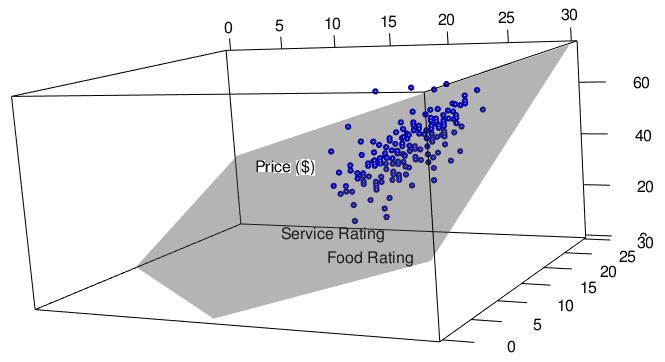
\includegraphics[width=0.5\textwidth]{figure/flatplane.png}
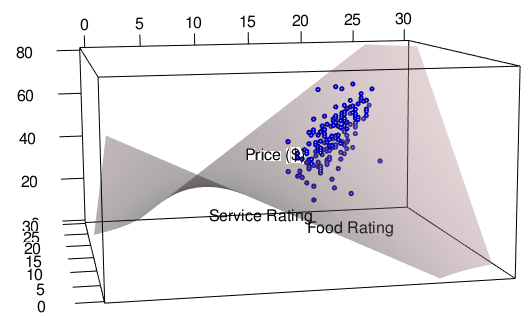
\includegraphics[width=0.5\textwidth]{figure/warpedplane.png}
\end{figure}

We were also talking about models with parallel planes and those with intersecting planes. 


\begin{Schunk}
\begin{Sinput}
> m.parallel <- lm(math~read+write+ses, data=hsb2)
> m.indep <-lm(math~read+write+ses+read*ses+write*ses, data=hsb2)
\end{Sinput}
\end{Schunk}


\begin{figure}[htbp]
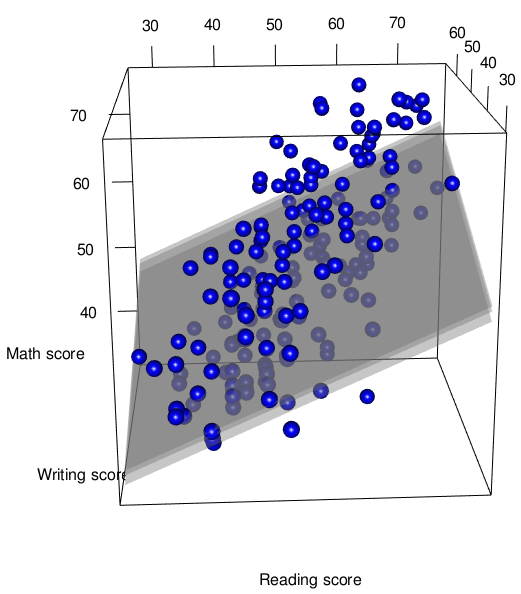
\includegraphics[width=0.5\textwidth]{figure/parallelplanes.png}
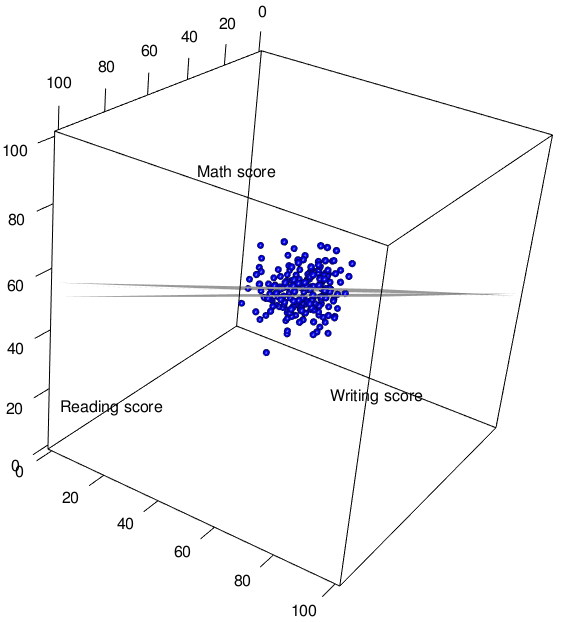
\includegraphics[width=0.5\textwidth]{figure/intersectingplanes.png}
\end{figure}

These plots have different shapes, depending on the way we choose to include terms in our model. Including a categorical variable can lead to parallel slopes or parallel planes, and an interaction between a categorical variable and a quantitative variable allows those lines or planes to have differnt slopes. Two quantative variables interacting leads to warped planes. But, what if a variable interacts with itself?

% \paragraph{Polynomial Regression}
% Consider the effect of interaction a variable could have \emph{with itself}! This yields a \emph{quadratic}, or \emph{second-order} model:
%    	$$
%   		Y = \beta_0 + \beta_1 X + \beta_2 X^2 + \epsilon
%    	$$
% 
% In general, we include lower-order terms even when not they are not statistically significant. This models extends to polynomial terms of arbitrary degree:
% 
%    	$$
%    		Y = \beta_0 + \beta_1 X + \beta_2 X^2 + \cdots + \beta_k X^k + \epsilon
%    	$$
% 
%   But we rarely use $k > 3$ in practice. A complete 2nd order model includes both quadratic and interaction terms:
%    	$$
%    		Y = \beta_0 + \beta_1 X_1 + \beta_2 X_2 + \beta_3 X_1 \cdot X_2 + \beta_4 X_1^2 + \beta_5 X_2^2 + \epsilon
%    	$$
% 
% 
% % The following activity will help you to think about which terms you will likely want to include in your model, based purely on \emph{reason}. 
% 
% When we have actual data, we can try many options, compare values of $R^2$, consider $p$-values for certain coefficients, and then make decisions about whether to include certain terms. But each term in the model equation above plays a certain role, and it doesn't always make sense to include all of the terms.
% 
% The roles of each term can be summarized as follows:
%    \begin{itemize}
%  		\item $\beta_0$: The constant term. This sets a typical value of $Y$, but doesn't depend on either $X_1$ or $X_2$. It is almost always included by default.
%  		\item $\beta_1 X_1$: The linear term in $X_1$. Produces a simple dependence on the input $X_1$; if the input $X_1$ changes, then the output $Y$ will change.
%  		\item $\beta_2 X_2$ Likewise, the linear term in $X_2$. This produces a simple dependence on the input $X_2$.
%  		\item $\beta_4 X_1^2$: The quadratic term in $X_1$ can do two things. It is absolutely needed in the model if there is a maximum or minimum with respect to $X_1$. But, even if there is no extremum, if there is an important change in $\frac{\Delta Y}{\Delta X_1}$ as $X_1$ changes, then there should be this quadratic term. Example: economists often speak of diminishing marginal returns -- doubling the amount of investment doesn't lead to a doubling in output per dollar of investment.
%  		\item $\beta_5 X_2^2$: The quadratic term in $X_2$. Like the quadratic term in $X_1$, it's needed for there to be an extremum with respect to $X_2$, or a change in $\frac{\Delta Y}{\Delta X_2}$.
%  		\item $\beta_3 X_1 X_2$: The interaction term. This term expresses how the inputs $X_1$ and $X_2$ interact: perhaps interfering with one another or reinforcing one another. Whenever the output will depend on $X_1$ differently for different values of $X_2$, or vice versa, there should be an interaction term included in the model.
%  	\end{itemize}

Almost always, we include the constant and linear terms in a model, although we might discover that they are not needed if other terms are added. The question is generally whether to include the quadratic and bilinear terms.

\begin{Schunk}
\begin{Sinput}
> require(mosaic)
> NYC <- read.csv("http://www.math.smith.edu/~bbaumer/mth241/nyc.csv")
> m1 <- lm(Price~Food, data=NYC)
> summary(m1)$adj.r.squared
\end{Sinput}
\begin{Soutput}
[1] 0.389528
\end{Soutput}
\begin{Sinput}
> mquad <- lm(Price ~ Food + I(Food^2), data=NYC)
> summary(mquad)
\end{Sinput}
\begin{Soutput}
Call:
lm(formula = Price ~ Food + I(Food^2), data = NYC)

Residuals:
     Min       1Q   Median       3Q      Max 
-21.2196  -4.6185   0.2306   3.9387  27.2306 

Coefficients:
            Estimate Std. Error t value Pr(>|t|)
(Intercept)  56.9185    53.1993   1.070    0.286
Food         -4.3853     5.1887  -0.845    0.399
I(Food^2)     0.1778     0.1257   1.414    0.159

Residual standard error: 7.239 on 165 degrees of freedom
Multiple R-squared:  0.4004,	Adjusted R-squared:  0.3932 
F-statistic:  55.1 on 2 and 165 DF,  p-value: < 2.2e-16
\end{Soutput}
\begin{Sinput}
> # same result, different code
> # lm(Price ~ poly(Food, 2, raw=TRUE), data=NYC)
> plotModel(mquad)
\end{Sinput}
\end{Schunk}


You don't want to go too crazy with polynomials, because you can end up overfitting your data. 


\begin{Schunk}
\begin{Sinput}
> # xyplot(y~x, data=d1, type=c("p", "r"), xlab="", ylab="")
> # mcube <- lm(y~poly(x, 3, raw=TRUE), data=d1)
> # plotModel(mcube, xlab="", ylab="")
> # mlots <- lm(y~poly(x, 26, raw=TRUE), data=d1)
> # plotModel(mlots, xlab="", ylab="")
> # summary(mlots)$r.squared
\end{Sinput}
\end{Schunk}



% \paragraph{Diagnostic Questions}
% 
% In order to decide which of these terms to include in a model for $Y$, it helps to ask the following questions about the quadratic terms and interaction terms:
% 
% 	\begin{enumerate}
% 		\item Is there an extremum with respect to $X_1$? That is, holding $X_2$ fixed, is there a value of $X_1$ at which $Y$ takes on a maximum or minimum value? If there is, you will want to include the quadratic term in $X_1$.
% 		\item If there is an extremum with respect to $X_1$, does its position or magnitude depend on the value of $X_2$? If so, include the interaction term.
% 		\item If there isn't an extremum with respect to $X_1$, does the rate of change with respect to $X_1$ depend on $X_2$? If so, include the interaction term even though there isn't a quadratic term in $X_1$.
% 		\item The same questions should be asked with respect to $X_2$ to decide whether to include the quadratic term in $X_2$.
% 		\item Both $X_1$ and $X_2$ participate in the interaction term, but sometimes one of the variables gives you a clearer indication that an interaction is important. Include it if warranted for either of the variables $X_1$ and $X_2$.
% 	\end{enumerate}

% \paragraph{Activity}
% 
% Decide which terms should be included in local models in these situations:
% \begin{enumerate}
%   \itemsep0.5in
% 	\item Economic production: The output of a factory, $P$, depends both on the amount of capital $C$ and the amount of labor $L$. What terms should be included in $P \sim (C, L)$?
% 	\item Infectious disease: The number of people $N$ who get an illness such as the flu depends on both the number of
% people who already have the illness $I$, and the number who are susceptible $S$. What terms should be included
% in $N \sim (S, I)$?
% 	\item Survival of chicks: The number of surviving fledglings $F$ of a mother bird depends on the number of eggs $N$ that are laid and the time that the mother spends collecting food $T$. What terms should be included in $F \sim (N, T)$?
% 	\item Day length: The length of daylight $D$ depends on both the time of the year $M$ (for month) and the latitude $L$. What terms should be included in $D \sim (M, L)$?
% 	\item Growth of a crop: The yield $Y$ of a crop (bushels/acre) depends both on the amount of water applied ($W$,
% inches/acre) and the amount of fertilizer ($F$, lbs/acre). What terms should be included in $Y \sim (W, F)$?
% 	\item Probability of admission to college: The probability $p$ that an applicant will be admitted to college depends on many things, but we will restrict consideration here to the math $M$ and verbal $V$ scores on an entrance examination such as the ACT or SAT. What terms should be included in $p \sim (M, V)$?
%   \vspace{0.2in}
% \end{enumerate}
% 
% We can generalize this approach to more than two variables. Here is a function of (at least) three variables.
% 
% \begin{itemize}
% 	\item Probability of a heart attack: The probability of a heart attack $p$ as a function of age $A$ and amount of exercise $E$, and number of calories in the diet $C$. What terms should be included in $p \sim (A, E, C)$?
% \end{itemize}




% \paragraph{Added Variable Plots}
% Added variable plots let us assess how much additional explanatory power a new variable has.
% 
% 	\begin{itemize}
% 		\item Procedure for analyzing an additional variable $Z$
% 		\begin{enumerate}
% 			\item Find residuals $\epsilon_1$ from $Y \sim X_1 + \cdots + X_k$
% 			\item Find residuals $\epsilon_2$ from $Z \sim X_1 + \cdots + X_k$ (modeling the new variable by all the previous variables)
% 			\item Plot $\epsilon_1 \sim 0 + \epsilon_2$ and investigate the slope. This shows the new variability in $Y$ that is explained by $Z$
% 		\end{enumerate}
%   \end{itemize}
% 
% Some properties of added variable plots:
%   \begin{itemize}
% 		\item Slope of regression line for residuals model is equal to $\beta_i$ in model for $Y \sim Z + \sum_j X_j$
% 		\item $(0,0)$ is ensured by zero mean of residuals
		% \item Consider our usual multiple regression model:
		% $$
		% 	Y \sim \beta_0 + \beta_1 X_1 + \cdots + \beta_k X_k + \epsilon \Rightarrow Y = \mathbf{X} \beta + \epsilon_{YX}
		% $$
		% \item Consider the addition of a new explanatory variable $Z$, such that
		% $$
		% 	Y = \mathbf{X} \beta + Z \alpha + \epsilon_{YXZ}
		% $$
		% \item Then, if $H_X = X(X^TX)^{-1} X^T$,
		% $$
		% 	\hat{\epsilon}_{ZX} = Z - \hat{Z} = Z - H_X Z = (I-H_X)Z
		% $$
		% \item But then,
		% \begin{align*}
		% 	\hat{\epsilon}_{YX} &= Y - \hat{Y} = Y - H_X Y = (I - H_X)Y \\
		% 	&= (I - H_X) (\mathbf{X} \beta + Z \alpha + \epsilon_{YXZ}) \\
		% 	&= (I - H_X) Z \alpha + (I-H_X) \epsilon_{YXZ} \\
		% 	&= \hat{\epsilon}_{ZX} \alpha + (I-H_X) \epsilon_{YXZ} \\
		% \end{align*}
%	\end{itemize}



\end{document}
